\documentclass{emonides-cv}
\usepackage{fontspec}

\setsansfont{Dotum}

\begin{document}
  
\rhead {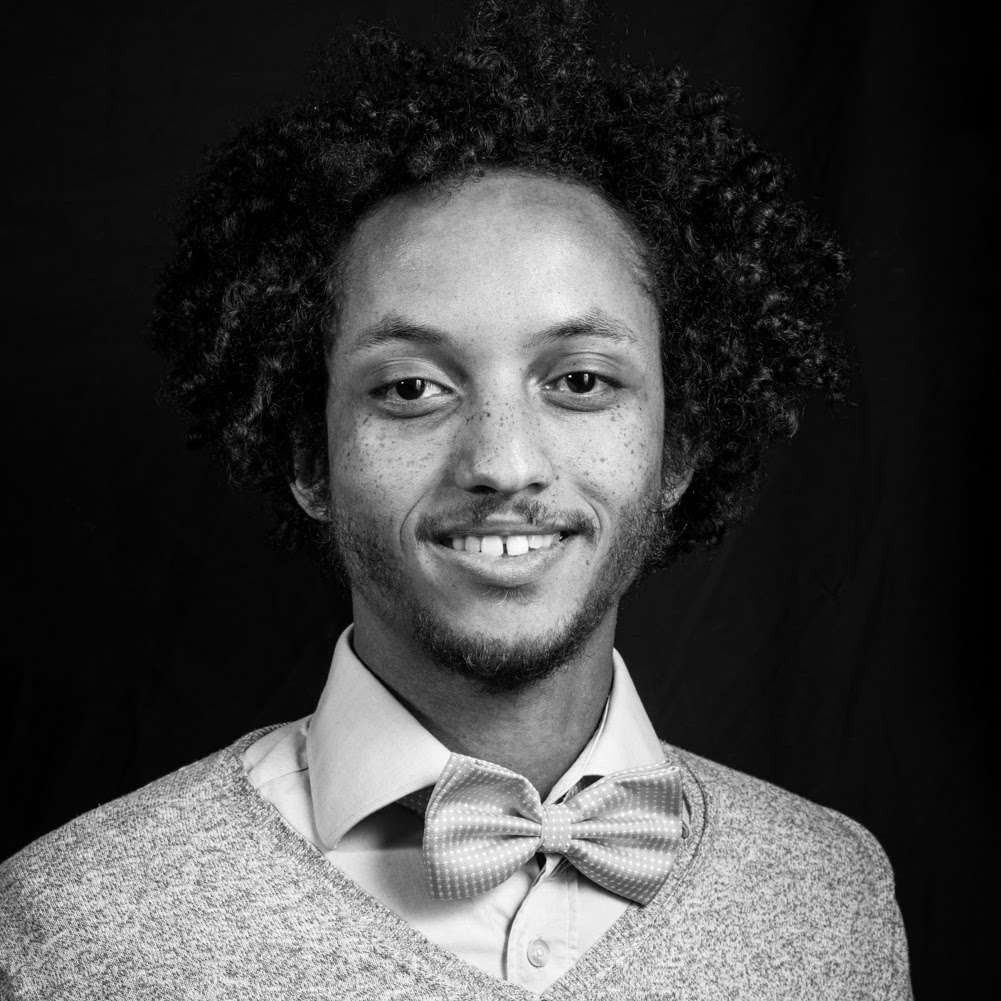
\includegraphics[width=1.5cm]{photoCV.jpg}}
  {Emonides} {Pierre-Emmanuel}  {Software Engineer/DevOps/MobileDeveloper}

\begin{aside}
  \section{about}
    130 Rue de Tolbiac
    75013 Paris
    France
    +33 665 44 88 14
    ~
  \section{languages}
    french native
    english fluent
    korean notions
  \section{misc}
    Driver Licence
\end{aside}

\section{Experience}
\begin{entrylist}
  \entry
    {Since  2016}
    {CTO at 360Boost {\normalfont Paris}}
    {Full Time}
    {\emph{Technical-lead, conception, planning, development and deployment of \textbf{C\# Android/IOS app, NodeJs} Servers.
     Managment of Clusters on \textbf{Gcloud, Kubernetes, Ansible}. Team-lead with 4 employees.}}
  \entry
    {March 2015}
    {Mobile Consultant, \href{https://www.docapost.com/en/}{Docaposte} {\normalfont Paris, La Défense}}
    {FullTime}
    {\emph{\textbf{Android/Java Developer}. Sent to a major client of Acensi Docapost, I had to develop on Java/Tomcat servers, as well as mobile applications on \textbf{Java Android}.}}
  \entry
    {Mars 2014-2015}
    {C\# Consultant, \href{https://www.acensi.fr/}{Acensi} {\normalfont Paris, La Défense}}
    {Intern then Fulltime}
    {\emph{\textbf{C\# WPF .Net4.5} development for a Finance Banquing software \href{https://www.eurocaution.net/}{Eurocaution}.
    I became team-lead for this project (15 developers, 3 teams).
    Then \textbf{C\# Xamarin} Mobile development on a para-medical application. \href{http://www.triacys.com/}{Triacys}.
    I worked on a custom Android Kernel for BeagleBoard, then Android Tablets. I also developped custom userspace-drivers for devices like blood pressure monitor.}}
  \entry
    {May-August 2012}
    {QT/C++ developer, \href{https://www.acensi.fr/}{Sogeti High Tech} {\normalfont Rennes}}
    {Intern}
    {\emph{\textbf{C++/QT} Developer for an IHM testing solution \href{https://www.eurocaution.net/}{Takt Engine}.
    I had to extend the capabilities of the testing solution. I worked with \textbf{OpenCV} to detect Bad Artefacts during Tests }}
  \entry
    {July-December 2010}
    {Lua GameDeveloper, \href{https://www.giantbomb.com/white-birds-productions/3010-5637/}{White Birds} {\normalfont Paris, La Défense}}
    {Intern}
    {\emph{Lua Developer for Point-and-click games, \href{https://www.bigfishgames.com/games/6859/cardboard-castle/}{Cardboard Castle}. \href{https://www.wikiwand.com/fr/White_Birds_Productions}{Last King of Africa}}}
\end{entrylist}

\section{Interests}
  \textbf{C\#, JavaScript, Python} , Java\\
  \textbf { NodeJS, Mobile Development, Xamarin.Forms/Android, WPF/WCF}  \\
  MongoDb, PostgreSQL, MySql\\
  \textbf { Ansible, Kubernetes, Docker}, Nginx, (Arch)Linux/*Bsd \\
  Google Cloud, Azure \\
  Git Workflow, Svn, Jira, Mantis\\
  \LaTeX, Gimp, Photoshop, 3DSMax\\
  \textbf { Certifications: 70-483 Programming in C\# }

\section{Education}
\begin{entrylist}
  \entry
    {2013-2014}
    {Master2 {\normalfont  Expert of Information Technologies }}
    {Epitech European Institute of Information Technology, Paris} {Project-oriented pedagogy : around 40 projects achieved alone or within a team.}
  \entry
    {2012-2013}
    {Master1 {\normalfont  Mobile\&Game development }}
    { {\sffamily 계명대학교} Keimyung University, Daegu South Korea} {}
  \entry
    {2009–2012}
    {Bachelor  {\normalfont Computer Science Programming and software design}}
    {Epitech, Rennes} {}
  \entry
    {2006–2009}
    {French Baccalauréat ES. {\normalfont with honors. }}
    {Lycée Schœlcher, Fort-de-France} { Specialization in mathematics }
\end{entrylist}

\section{Activities}
  Thai boxing, Underwater diving\\
  3D Modeling, Drawing\\
  Skating, MotorBike
  
\end{document}

